\documentclass{beamer}
\usepackage[utf8]{inputenc}
\usepackage{amsmath}
\usepackage{graphicx}
\usepackage{xcolor}
\usepackage{tikz}
\usepackage{listings}
\lstset{
    basicstyle=\small\ttfamily,
    breaklines=true,
    showstringspaces=false,
    commentstyle=\color{gray},
    keywordstyle=\color{blue}
}
\usetheme{Madrid}
\usecolortheme{default}

% Define custom colors inspired by Star Trek DS9
\definecolor{ds9blue}{RGB}{25,25,112} % Midnight Blue
\definecolor{ds9gold}{RGB}{218,165,32} % Goldenrod
\definecolor{ds9grey}{RGB}{105,105,105} % Dim Gray
\definecolor{ds9red}{RGB}{178,34,34} % Firebrick

% Customize the colors
\setbeamercolor{title}{fg=ds9gold}
\setbeamercolor{frametitle}{bg=ds9blue, fg=white}
\setbeamercolor{block title}{bg=ds9gold, fg=black}
\setbeamercolor{block body}{bg=ds9grey!20, fg=black}
\setbeamercolor{section in toc}{fg=ds9gold}
\setbeamercolor{subsection in toc}{fg=ds9gold!70}
\setbeamercolor{footline}{bg=ds9blue, fg=white}
\setbeamercolor{author in head/foot}{fg=white}
\setbeamercolor{date in head/foot}{fg=white}
\setbeamercolor{title in head/foot}{fg=white}

% Title page configuration
\title[Recursive Sequences \& Functions]{Introduction to Recursive Sequences and Functions}
\subtitle{Understanding Recursion in Mathematics and Programming}
\author[Mr. Gullo]{}
\date[Nov 2024]{November 2024}



\AtBeginSection[]
{
  \begin{frame}
    \frametitle{Table of Contents}
    \tableofcontents[currentsection]
  \end{frame}
}

\begin{document}

\frame{\titlepage}

\section{Introduction to Recursion}


\begin{frame}
\begin{figure}
    \centering
    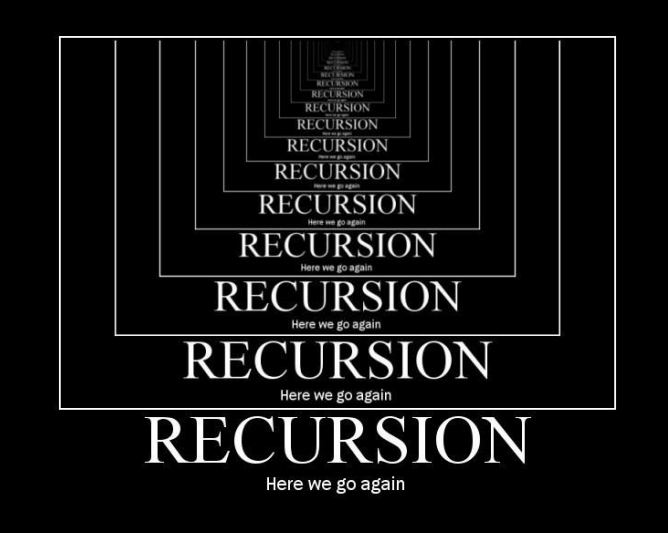
\includegraphics[width=1\linewidth]{CS12Recursive Functions/Screenshot 2024-11-11 150024.png}
\end{figure}
    
\end{frame}

\begin{frame}
\frametitle{What is Recursion?}
\begin{itemize}
    \item A process where the definition refers to the thing being defined
    \item Example: The Sleeping Story
    \begin{itemize}
        \item A child couldn't sleep, so mother told a story about...
        \item a frog who couldn't sleep, so its mother told a story about...
        \item a bear who couldn't sleep, so its mother told a story about...
        \item a weasel
        \item ...who fell asleep.
        \item ...and the little bear fell asleep;
        \item ...and the little frog fell asleep;
        \item...and the child fell asleep.
    \end{itemize}
\end{itemize}
\end{frame}
\begin{frame}{Recursive Functions}
\begin{figure}
    \centering
    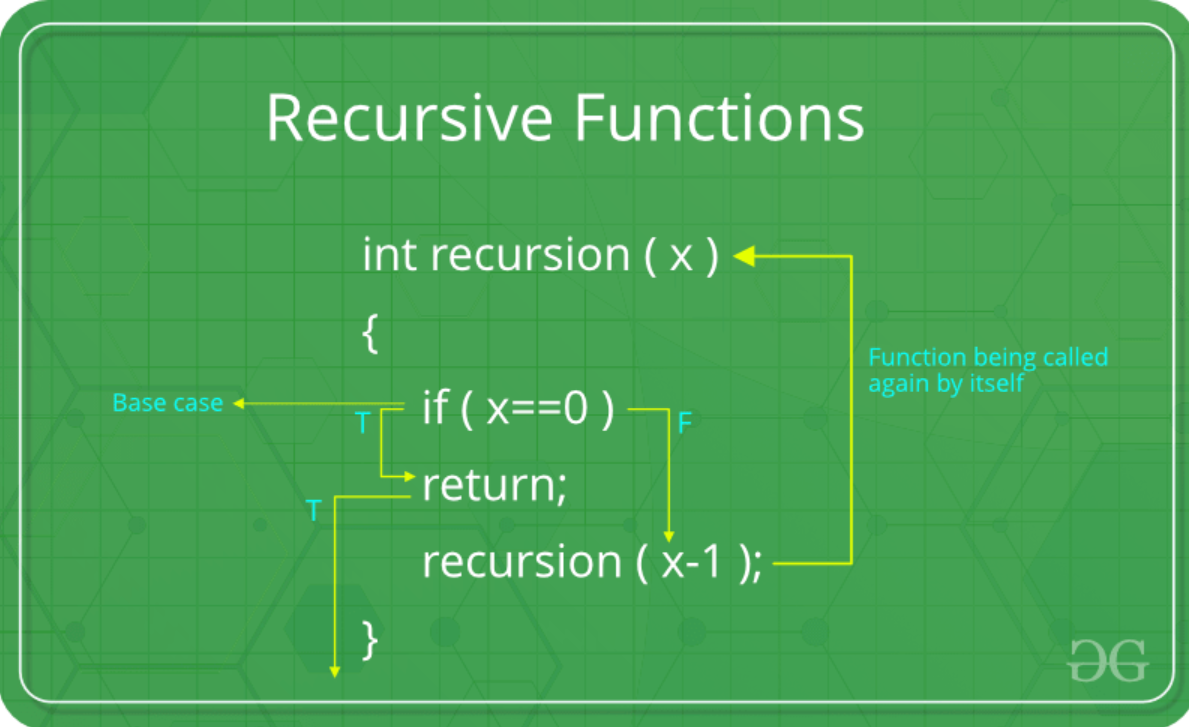
\includegraphics[width=1\linewidth]{CS12Recursive Functions/Screenshot 2024-11-11 152930.png}
\end{figure}
    
\end{frame}
\section{Recursive Sequences}

\begin{frame}
\frametitle{Recursive Sequences: Basic Form}
\begin{itemize}
    \item A recursive sequence is defined by:
    \begin{itemize}
        \item Initial term(s)
        \item A rule for finding subsequent terms
    \end{itemize}
    \item General Form for Geometric Sequences:
    \[ t_n = t_1r^{n-1} \]
    where:
    \begin{itemize}
        \item $r$ is the common ratio
        \item $r = \frac{t_i}{t_{i-1}}$ for $i > 1$
    \end{itemize}
\end{itemize}
\end{frame}

\begin{frame}
\frametitle{Types of Recursive Rules}
\begin{block}{Simple Recursive Rule}
\[ t_n = \begin{cases} 
t_1 = 1 \\
t_n = t_{n-1} + 1
\end{cases} \]
\end{block}

\begin{block}{Multiple Term Dependencies}
\[ t_n = \begin{cases}
t_1 = t_2 = 1 \\
t_n = t_{n-1} + t_{n-2} \text{ (Fibonacci)}
\end{cases} \]
\end{block}
\end{frame}

\begin{frame}
\frametitle{Common Examples}
\begin{enumerate}
    \item Arithmetic: $a_n = a_{n-1} + d$
    \item Geometric: $a_n = a_{n-1} \cdot r$
    \item Fibonacci: $a_n = a_{n-1} + a_{n-2}$
    \item Complex: $a_n = n + a_{n-1} + 6$
\end{enumerate}
\end{frame}

\section{Programming with Recursion}

\begin{frame}
\frametitle{Common Programming Exercises}
\begin{itemize}
    \item Fibonacci Sequence Implementation
    \item Counting Digits Recursively
    \item Sum of Digits Using Recursion
    \item Binary Conversion
    \item Greatest Common Factor (GCD)
    \item Lowest Common Multiple (LCM)
\end{itemize}
\end{frame}

\begin{frame}[fragile]
\frametitle{Common Mistake 1: Forgetting Base Cases}
\begin{columns}
\begin{column}{0.48\textwidth}
\begin{block}{Incorrect}
\begin{lstlisting}[language=C++]
int factorial(int n) {
    return n * factorial(n - 1);
}
\end{lstlisting}
\end{block}
\end{column}

\begin{column}{0.48\textwidth}
\begin{block}{Correct}
\begin{lstlisting}[language=C++]
int factorial(int n) {
    if (n == 0) 
        return 1;
    return n * factorial(n - 1);
}
\end{lstlisting}
\end{block}
\end{column}
\end{columns}
\end{frame}

\begin{frame}[fragile]
\frametitle{Common Mistake 2: Infinite Recursion}
\begin{columns}
\begin{column}{0.48\textwidth}
\begin{block}{Incorrect}
\begin{lstlisting}[language=C++]
int countDown(int n) {
    cout << n << " ";
    return countDown(n - 1);
}
\end{lstlisting}
\end{block}
\end{column}

\begin{column}{0.48\textwidth}
\begin{block}{Correct}
\begin{lstlisting}[language=C++]
int countDown(int n) {
    if (n < 0) 
        return 0;
    cout << n << " ";
    return countDown(n - 1);
}
\end{lstlisting}
\end{block}
\end{column}
\end{columns}
\end{frame}

\begin{frame}[fragile]
\frametitle{Common Mistake 3: Stack Overflow}
\begin{columns}
\begin{column}{0.48\textwidth}
\begin{block}{Incorrect}
\begin{lstlisting}[language=C++]
int fibonacci(int n) {
    return fibonacci(n-1) 
        + fibonacci(n-2);
}
\end{lstlisting}
\end{block}
\end{column}

\begin{column}{0.48\textwidth}
\begin{block}{Correct}
\begin{lstlisting}[language=C++]
int fibonacci(int n) {
    if (n <= 1) 
        return n;
    return fibonacci(n-1)
        + fibonacci(n-2);
}
\end{lstlisting}
\end{block}
\end{column}
\end{columns}
\begin{alertblock}{Stack Overflow Explained}
Each recursive call adds a new layer to the program's memory stack, and without proper base cases, these layers pile up until the computer runs out of memory space.
\end{alertblock}
\end{frame}

\begin{frame}[fragile]
\frametitle{Common Mistake 4: Incorrect Recursive Step}
\begin{columns}
\begin{column}{0.48\textwidth}
\begin{block}{Incorrect}
\begin{lstlisting}[language=C++]
int sum(int n) {
    if (n == 0) 
        return 0;
    return n + n-1; // Wrong!
}
\end{lstlisting}
\end{block}
\end{column}

\begin{column}{0.48\textwidth}
\begin{block}{Correct}
\begin{lstlisting}[language=C++]
int sum(int n) {
    if (n == 0) 
        return 0;
    return n + sum(n-1);
}
\end{lstlisting}
\end{block}
\end{column}
\end{columns}
\end{frame}

\begin{frame}[fragile]
\frametitle{Common Mistake 5: Edge Cases in Recursion}
\begin{alertblock}{Key Point}
Always check the input's validity before processing!
\end{alertblock}

\begin{columns}
\begin{column}{0.48\textwidth}
\begin{block}{Missing Edge Case}
\begin{lstlisting}[language=C++]
int countDown(int n) {
    cout << n << " ";
    return countDown(n-1);
}
\end{lstlisting}
\end{block}
\end{column}

\begin{column}{0.48\textwidth}
\begin{block}{With Edge Case}
\begin{lstlisting}[language=C++]
int countDown(int n) {
    if (n < 0) return 0;
    cout << n << " ";
    return countDown(n-1);
}
\end{lstlisting}
\end{block}
\end{column}
\end{columns}
\end{frame}

\section{Practice Problems}

\begin{frame}
\frametitle{Exercise Types}
Write the first 5 terms for sequences with rules like:
\begin{enumerate}
    \item $a_1 = 4$ and $a_n = n + a_{n-1} + 6$
    \item $a_1 = 0$ and $a_n = a_{n-1} - n^2$
    \item $a_1 = 2$ and $a_n = (a_{n-1})^2 + 2$
\end{enumerate}
\end{frame}

\begin{frame}
\frametitle{Real-World Application}
\begin{example}[Swimming Pool Problem]
You add chlorine to a pool:
\begin{itemize}
    \item First week: 750mL
    \item Every week after: 350mL
    \item 40\% evaporates each week
\end{itemize}
Write a recursive rule for the amount of chlorine each week.
\end{example}
\end{frame}

\section{Advanced Topics}

\begin{frame}
\frametitle{Piece-wise Recursive Rules}
Example:
\[ a_n = \begin{cases}
7 & \text{if } n = 1 \\
\frac{a_{n-1}}{2} & \text{if } a_{n-1} \text{ is even} \\
3a_{n-1} + 1 & \text{if } a_{n-1} \text{ is odd}
\end{cases} \]
\end{frame}

\begin{frame}
\frametitle{Explicit vs. Recursive Rules}
\begin{columns}
\column{0.5\textwidth}
Explicit Rule:
\[ t_n = n \]

\column{0.5\textwidth}
Recursive Rule:
\[ t_n = \begin{cases}
t_1 = 1 \\
t_n = t_{n-1} + 1
\end{cases} \]
\end{columns}
\end{frame}

\begin{frame}
\frametitle{Conclusion}
\begin{itemize}
    \item Recursion is a powerful mathematical and programming tool
    \item Key concepts:
    \begin{itemize}
        \item Base cases
        \item Recursive steps
        \item Multiple approaches (explicit vs. recursive)
    \end{itemize}
    \item Practice with both mathematical and programming problems
\end{itemize}
\end{frame}

\end{document}